\documentclass[11pt,letterpaper]{article}
\usepackage[latin1]{inputenc}
\usepackage{amsmath}
\usepackage{amsfonts}
\usepackage{amssymb}
\usepackage{url}
\usepackage{graphicx, fullpage}
\author{J. Decker}
\date{17 March 2012}
\title{Ground Test of xBee Radios}
\begin{document}
\maketitle
\begin{abstract}
A second range test was conducted.  Demonstrated a usable range of 600m in an austere RF environment.
\end{abstract}

\section{Objective and Success Criteria}
\begin{description}
\item[Objective:] Demonstrate the conservative useful range of xBee Pro radios and 2dBi antennas.
\item[Success Criteria:] Transmit and receive packets at 600 meters range; observe received signal strength indication of the remote radio.
\end{description}

\section{Setup}

The setup of the 26 Feb tests\footnote{rangeTests26Feb2012.pdf} was duplicated with two important differences: 1) The radio fastened to the window was seated on Adafruit's xBee adapter, powered with 5V (from a power supply), with the Tx and Rx pins shorted; 2) the remote unit was powered from a Sparkfun USB board plugged into a laptop running Digi's X-CTU software.

The remote radio was then driven away while watching the lost and received packet counters.  The remote radio was driven to a line of sight distance of $\sim$600m; see Figure \ref{googleMaps}.  At range, the antenna was held out of the sunroof of the author's Acura. 


\begin{figure}[ht]
\begin{center}
%trim=<l> <b> <r> <t>
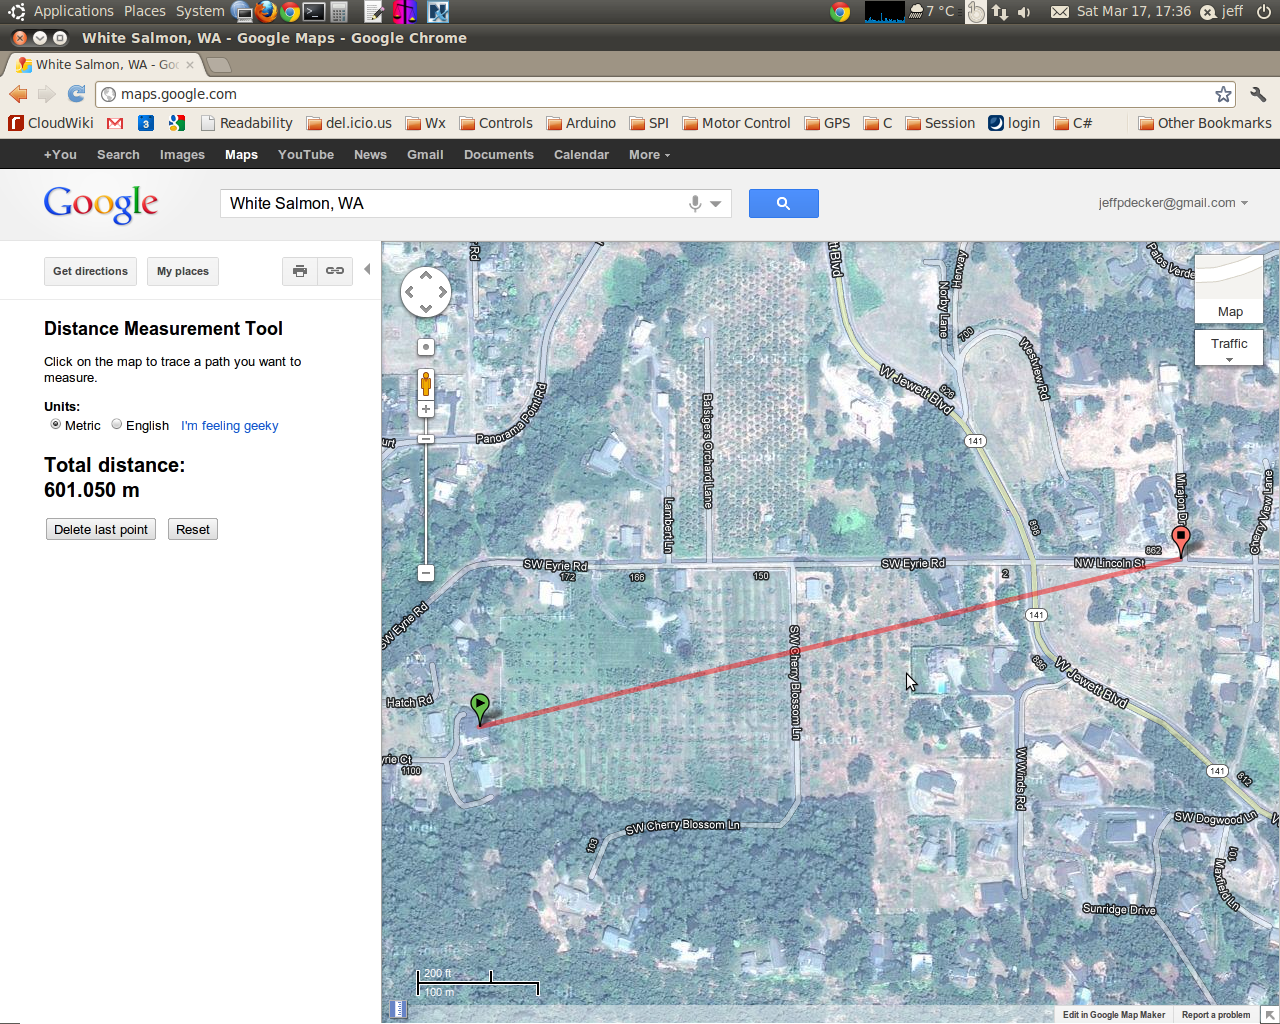
\includegraphics[scale=0.45, trim = 160mm 70mm 30mm 140mm, clip]{600mRangeTest.png}
\centering
\caption{Google maps view of line of sight range test.}
\label{googleMaps}
\end{center}
\end{figure}


\section{Results}

Again, the hardware and software setup were confirmed working at short ($\sim$5m) distance before beginning the drive away.  Again, the RSSI indicated in the X-CTU software was $\sim$84dB.

At the intersection of NW Lincoln St and Mirajon Dr, the remote radio reported a good percentage of received packets ($\sim$90\%), though the performance was extremely sensitive to antenna placement.  The antenna was oriented vertically, and moving it left or right a few centimeters changed the received/lost ratio dramatically.  The RSSI was not noted.

\section{Analysis}

Consistent with the 26 Feb range tests, the RSSI at close range should have been much higher.  During this test, both the base radio and remote radio were provided with known good 5V power, thus eliminating the idea that power to the radio may have been inadequate during the 26 Feb testing.

The 26 Feb testing questioned the radio performance in close proximity to cellphones; this round of testing did not involve the active use of cellphones; although two cellphones were in the car, no calls were placed.

At a range of 600m, the radios were able to successfully send and receive a series of packets.  Though the radios probably had line-of-sight, the space between the two antennas was not ``free space," but rather riddled with house roofs, and tree tops, etc, which would be detrimental to radio performance.  The remote radio was held flush with the 
roof of the Acura, possibly giving the remote radio the benefit of a generous ground plane.

Furthermore, the demonstrated distance would be exceedingly difficult for an aircraft to aircraft ``hit".  The required accuracy to hit within a 10m wingspan at 600m is less than 1$^\circ$ as given by:
\[\arctan (10/600) = 0.9548^\circ  \]


\section{Conclusion}

This range test demonstrated adequate radio performance at the edge of reasonable air-to-air combat range.  The range test of 26 Feb left open the question of adequate margin at 450m.  Because good radio performance was demonstrated at 600m in an austere RF environment, and because the radios' manufacturer specifies 3km range, adequate link margin is assumed.  

\section{Recommendations}
End range testing.

\end{document}